\subsubsection{Varsling}
Varsling er en funksjon i overvåkningsløsningen som krever en del finjusteringer og balansering av parametere over tid. Det vil være en balansegang med å varsle for mye og filtrere for grovkornet. Et tegn på et godt overvåknsingssystem er at det er fokusert, og ikke gir oveflødig mengde informasjon /cite  Building a Monitoring Infrastructure with Nagios . Dersom det ofte sendes ut “falske varsler” kan dette føre til at en alvorlig hendelse ikke blir oppdaget selv om det faktisk sendes ut varsel. Når varsler sendes ut er det til de som vil og trenger å få de.

\subsubsection{Avhengigheter}
For å holde antallet varsler som sendes ut nede benyttes avhengigheter som beskrevet i \ref{sec:servicedependency}  og \ref{sec:parent} for å ikke få mer enn en melding ved følgefeil. “Parent” har blitt benyttet til å reflektere det fysiske nettverksoppsettet. Service dependency-objekter er satt opp for noen tjenester. For eksempel tjenester som blir sjekket via NRPE vil være avhengig av at NRPE-daemonen på gitt host kan motta henvendelser.

\subsubsection{Konfigurasjon}
I Icinga kan man lage kontakter og legge disse i kontaktgrupper. Oppsettet følger samme logikk som at et hostgroup-objekt referer til en eller flere host-objekt i et service-objekt.
Det vil si at contact- og contactgroup-objekter refereres til i et service- eller host-objekt. Disse kontaktene kan bli varslet om service-objektet får en annen status enn OK. Dette konfigureres i service-objektet sammen ved hvilke tilstander som skal varsles. Disse tilstandene er vist i tabell \ref{notications}.

Når en feil oppstår vil Icinga vurdere ulike konfigurasjonsopsjoner før det eventuelt sendes ut et varsel. Om konfigurasjonsopsjonene tilsier at det skal varsles, vil Icinga gå igjennom filtre som er ferdig definert, som for eksempel om kontakten eller gruppen skal ha varsel via sms eller email. 

\begin{table}
\begin{center}
\begin{tabular}{| c | l | l | p{7cm} |}
        \hline
        \textbf{Objekt} & \textbf{Opsjon} & \textbf{Tilstand} & \textbf{Det sendes varsler om}
        \\ \hline
	\multirow{3}{*}{Host} & d & DOWN 			& Host-objektet er nede 			\\ \cline{2-4}
					    & u & UNREACHABLE 		& Et parent er nede eller unreachable.		\\ \cline{2-4}	
					    & r & UP 			& Hosten går til UP				\\ \hline 
        \multirow{3}{*}{Service} 	    & c & CRITICAL 		& Service-en er i CRITICAL 			\\ \cline{2-4}
					    & w & WARNING  		& Service-en er i WARNING  			\\ \cline{2-4}
					    & u & UNKNOWN  		& Service-en er i UNKNOWN  			\\ \hline
	\multirow{4}{*}{Host eller Service} & f & FLAPPING           	& Flapping starter eller slutter 		\\ \cline{2-4}
					    & s & Scheduled downtime 	& Planlagt nedetid starter eller slutter 	\\ \cline{2-4}
				 	    & r & UP                 	& Objektet går til UP 				\\ \cline{2-4}  
					    & n &                    	& Det skal ikke varsles ved noen tilfeller 	\\ \cline{2-4}

	\hline
\end{tabular}
\label{objekt_varsling}
\end{center}
\end{table}


\subsubsection{Flapping}
I Icinga defineres “flapping” som når et host- eller service-objekt skifter tilstand for ofte, noe som resulterer i mange problem- og recoveryvarsler. \cite{icingaflapping} Dersom detektering av flapping er konfigurert for objektet vil Icinga stoppe varsler for det dersom prosentandelen flapping overstiger en konfigurert grense. Objektet regnes som å ha startet å flappe når andelen for første gang overstiger en “høy”-grense og som å stoppe å flappe når andelen igjen er under en “lav”-grense.

Denne prosentandelen er kalkulert ved at
\begin{itemize}
	\item Lagrer resultatet for de siste 21 sjekkene.
	\item Finner når tilstandsendring skjer 
	\item Kalkulerer flap prosent ut fra andelen tilstandsendringer
	\item Vekter nyeste sjekker mer
\end{itemize}

Som standard er denne grensen satt til 20.0 for høy og 5 for lav i Icinga.cfg. Men den kan også konfigureres på hvert host- og service-objekt med direktivene “low\_flap\_threshold” og “high\_flap\_threshold”, som vist i eksempelet under:

\begin{lstlisting}
define host {
	name important_servers  		#template
	use generic_host
	flap_detection_enabled          1     ; Flap detection is enabled
	low_flap_threshold		70    ; Stop flapping at 70 %
	high_flap_threshold		80    ; Start flapping at 80 %
	register			0
}
\end{lstlisting}

\subsubsection{Oppsett av kontakter og kontaktgrupper}


IKT-avdelingen ønsket å kunne styre kontaktinformasjon og kontaktgrupper fra Active Directory. Det ble bestemt at ansvarsforhold skulle gjenspeiles i kontaktgrupper /ref vedlegg møte, for eksempel “ts\_ansvarlig” eller “printer\_ansvarlig”. Icinga støtter ikke integrasjon mot LDAP i konfigurasjonsfilene, men siden disse er rene tekstfiler kan de enkelt opprettes og endres med script. Vi var i utgangspunktet skeptiske til å la et script gjøre endringer i konfigurasjonsfiler, da vi var redd for at dette kunne medføre en konfigurasjon med feil, som igjen ville føre til at Icinga ikke ville kunne lese ny konfigurasjon. 

Icinga har en funksjon som gjør at en kan teste konfigurasjonen etter feil med en opsjon på binærfilen (--verify-config). Icinga vil da ta utgangspunkt i rot-konfigurasjonsfilen (icinga.cfg) for å sjekke alle konfigurasjonsfilene. Dette gjør at alle konfigurasjonsfilene må sjekkes og ikke bare de som lages for kontakter. Dermed vil ikke kontakter og kontaktgrupper bli oppdatert dersom det allerede er en feil i konfigurasjonen. 

Det ble skrivet et Perl-script (ref vedlegg X) som henter ut kontakter og kontaktgrupper fra en bestemt OU i Active Directory. Perl ble benyttet fordi det ble funnet et godt sett med LDAP-moduler, "perl-ldap" \cite{http://ldap.perl.org} som gjorde tilkobling og søk enkelt. Scriptet kalles fra et bash-script (ref vedlegg X) som henter resultatet fra synkroniseringen og sender dette til Icinga. En cron-jobb er satt opp for å kjøre synkroniseringen én gang i timen.

Måten scriptet fungere på:
\begin{enumerate}
	\item Henter alle medlemmer av gruppe “icinga\_kontakter” og medlemmer av grupper som er medlem.
	\item Oppretter en konfigurasjonsfil for hver av medlemmene.
	\item Henter alle grupper under “Kontaktgrupper”.
	\item Henter alle grupper under “Kontaktgrupper”.
	\item Det opprettes en egen service-template der kontaktgruppen er satt til å få meldinger, slik at tjenester kan arve fra denne.
\end{enumerate}

\makeatletter
\newcount\dirtree@lvl
\newcount\dirtree@plvl
\newcount\dirtree@clvl
\def\dirtree@growth{%
  \ifnum\tikznumberofcurrentchild=1\relax
  \global\advance\dirtree@plvl by 1
  \expandafter\xdef\csname dirtree@p@\the\dirtree@plvl\endcsname{\the\dirtree@lvl}
  \fi
  \global\advance\dirtree@lvl by 1\relax
  \dirtree@clvl=\dirtree@lvl
  \advance\dirtree@clvl by -\csname dirtree@p@\the\dirtree@plvl\endcsname
  \pgf@xa=0.5cm\relax
  \pgf@ya=-0.5cm\relax
  \pgf@ya=\dirtree@clvl\pgf@ya
  \pgftransformshift{\pgfqpoint{\the\pgf@xa}{\the\pgf@ya}}%
  \ifnum\tikznumberofcurrentchild=\tikznumberofchildren
  \global\advance\dirtree@plvl by -1
  \fi
}

\tikzset{
  dirtree/.style={
    growth function=\dirtree@growth,
    every node/.style={anchor=north},
    every child node/.style={anchor=west},
    edge from parent path={(\tikzparentnode\tikzparentanchor) |- (\tikzchildnode\tikzchildanchor)}
  }
}
\makeatother
\begin{document}
\begin{tikzpicture}[dirtree]
\node {OU: icinga\_kontakter}
    child { node {Gruppe: alle\_kontakter} }
    child { node {OU: Kontaktgrupper}
        child { node {Gruppe: ts\_ansvarlig} }
        child { node {Gruppe: exchange\_ansvarlig} }
        child { node {Gruppe: mysql\_cluster\_ansvarlig} }
    }
\end{tikzpicture}

For hver gang en konfigurasjonsfil skrives blir det først tatt en backup dersom en fil med gruppe- eller kontaktnavnet finnes fra før. Etter at den nye filen er skrevet, sjekkes konfigurasjonen og dersom det oppdages feil vil backupen bli kopiert tilbake. 

Til slutt sendes resultatet som en passiv sjekk til Icinga. Dersom ingen feil oppstår sendes OK. Hvis ikke vil det gis en CRITICAL der feilmeldingene blir sendt med som resultat av sjekken. Det sjekkes også om e-post-adresse og mobilnummer er definert for alle kontakter. Hvis dette ikke  er satt vil det gis en WARNING på service-objektet “Contact sync” i Icinga.

For å sikre at synkroniseringen kjører er service-objektet satt opp med en freshness-sjekk. Dette vil si at det forventes at Icinga mottar et resultat av sjekken hver time (pluss en feilmargin på 1 minutt). Dersom det ikke skjer vil det bli satt en feil på “Contact sync”. Konfigurasjonen for service-objektet er vist under:
\begin{lstlisting}

define service contact_sync {
   use 				generic_service
   host_name      		localhost
   service_description  	Contact sync
# Only use passive checks for this service
   active_checks_enabled   	0
   passive_checks_enabled  	1
   check_freshness      	1
   freshness_threshold     	3660 ; 1h + 1 min splay time
# if we don't get a passive result within freshness_threshold this will be run
   check_command     		check_dummy!2 "No contact sync has been run for 24hrs" 
}
\end{lstlisting}

\subsubsection{Timeperiod}

Objektettypen timeperiod er sterkt knyttet til kontakter. Her kan en definere perioder for varsling. En har mulighet til å definere spesifikke dager, datoer eller hver n-te dag. 

Det var ønskelig at det ikke skulle sendes ut varsler når IKT-avdelingen har servicevindu, den første onsdagen etter andre tirsdagen i hver måned (dagen etter Patch-Tuesday fotnote \cite{wiki:patch}). For å få til dette ble det først prøvd å definere det slik:

\begin{lstlisting}
define timeperiod {
	tuesday 2 +1       15:00-04:00
}
\end{lstlisting}

Dette fungerte imidlertid ikke. Løsningen ble å definere perioden for tirsdagen og onsdagen, for så å ekskludere tirsdagen. Slik:
\begin{lstlisting}
define timeperiod {
        timeperiod_name 	patch_tuesday
        alias           	Patch tuesday
        tuesday 2          	00:00-24:00  ;second tuesday of every month
}
\end{lstlisting}

\begin{lstlisting}
define timeperiod {
        timeperiod_name         service_vindu
	 alias			Servicevindu
        tuesday 2 - wednesday   15:00-04:00
        exclude patch_tuesday
}
\end{lstlisting}

\subsubsection{Eskalering}

Når varsel har blitt sendt ut, og tilstanden til et host- eller service-objekt ikke har endret seg over en definert tidsperiode, kan et eskalerings varsel sendes. Contact- eller contactgroup-objektene som er referert til i et host- eller serviceescalation-objekt, vil da motta SMS eller e-mail om hendelsen .

Et eksempel på når dette kan være nyttig er om ledere for et driftsteam ønsker å bli varslet dersom temperaturen på serverrommet fortsatt ligger over varselsgrensen etter at 10 varsler er sendt ut til ansvarlige for kjølingen. Her får lederen mulighet til å ta nødvendige avgjørelser for at problemet skal løses. Dette er vist under:
\begin{lstlisting}
define serviceescalation {
	hostgroup_name		temperature_sensors
	service_description	Check Temperature
	contact_groups		team_leaders
	first_notification	10	# Ten notifications has to be sent before escalation
	last_notification	15	# After fiftheen notifications, this escalation stops. "0" is forever.
	notification_interval	60 	# Escalation notifications are sent every 60 minutes (default 45)
	escalation_options	c	# Only use escalation when service  is C(ritical)
	escalation_period	op_hours  # Only escalate during hours of operations
}
\end{lstlisting}
Det samme kan benyttes på host-objekter ved at ikke service\_description defineres:
\begin{lstlisting}
define hostescalation {
	hostgroup_name		domain_controllers
	contact_groups		big_bosses
	first_notification	3 	last_notification	5 # When does escalation notifications stop
	notification_interval	50
	escalation_options	d #Only use escalation when host is D(own)
}
\end{lstlisting}

\subsubsection{Varslingsmelding}\label{sec:varslingsmelding}

Selve varslingsmeldingene sendes ut først når host- eller service-objekter er i en hard tilstand (beskrevet i \ref{sec:sjekker}). Et eksempel er om en brannmurs hostsjekk returnerer DOWN. Da er det ikke ønskelig å varsle over SMS eller e-post, dersom det er snakk om et par ping som mistes. For eksempel kan en sjekk som har returnert DOWN kjøres to ganger til, med et intervall på ett minutt, før en hard tilstand settes, slik:

\begin{lstlisting}
define host {
   use 	generic_host     # Inherit basic config. check_ping for host_check
   host_name	hig-fw1
   max_check_attempts           2 # Number of checks before hardstate
    retry_check_interval        1 # 60 seconds between each consecutive check
}
\end{lstlisting}

For et contact-objekt kan det settes opp ett eller flere command-objekt for både hosts og servicer som skal brukes for utsending og formatering av varslingsmeldingen.  

I eksempelet under brukes command-objektet notify-host-by-email og notify-host-by-sms for varslingsmeldinger:
\begin{lstlisting}
define contact {
   contact_name Kari Sysadmin
   email kari@company.org
   pager 480 88 256 
   host_notification_commands    host_problem_email, host_problem_sms
   service_notification_commands service_problem_email, service_probleml_sms
}
\end{lstlisting}

I eksempelet under vises et command-objekt fra selve implementasjonen. Her benyttes sendmail \cite{wiki:sendmail} til å sende en epost til en SMS-gateway.

\begin{lstlisting}
define command {
   command_name host_problem_sms
   command_line /usr/bin/printf "%b" "Subject:$CONTACTPAGER$\n***** Icinga *****\n\nHost: $HOSTNAME$\nAddress: $HOSTADDRESS$\nState: $HOSTSTATE$\nTime: $SHORTDATETIME$\nInfo: $HOSTOUTPUT$" | /usr/sbin/sendmail -f icinga@hedmark.org -v $CONTACTPAGER$@smsgw.sms
}
\end{lstlisting}

Varslingsmelder som sendes over SMS vil være korte og lettfattede, mens de som sendes til e-post gjerne er lengre og inkluderer mer utfyllende informasjon. Informasjonen som sendes ut hentes ut ved hjelp av makroer i Icinga \cite{icingamacro}. 

Alle varslingsmeldinger sendes fra en og samme e-post-server. Dette er ikke helt ideelt fordi en vil miste både SMS- og e-postvarsling, dersom e-post-serveren skulle slutte å fungere. Løsningen vil være å definere en fallback-server som ble brukt hvis Icinga ikke får kontakt med e-post-serveren. 

\subsubsection{Kritisk Varsling}

For kritiske tjenester og utstyr er det i konfigurasjonen defineret et eget generisk objekt som brukes av de service- og host-objektene som anses som kritiske. Dette gjelder domenekontrollere, nettverksutstyr på hoveddatarommet, temperatursensorer og UPS-er. Disse objektene vil sjekkes oftere enn det som er satt som standard. Varslingsmelding vil også sendes til alle ved IKT-avdelingen om en hendelse skulle inntreffe, også utenom arbeidstid og i servicevinduet.

\subsubsection{Statusvisning}

Icinga har allerede som nevnt i \ref{sec:teoriweb} et webgrensesnitt. Dette er et verktøy for å utføre handlinger på hosts og servicer. Her finnes også et “tactical overview”, som vist i Figur \ref{icingawebgui}. Det er ikke tilrettelagt for å få vist en kort, og beskrivende beskjed om hva som er galt på de host-ene og tjenestene med feil på en stor skjerm. Det vises et antall for de ulike statusene, men her krever det flere handlinger for å få en bedre oversikt, og er tilrettelagt for administrering. Det ble derfor besluttet å utvikle et webgrensesnitt som er tilpasset IKT-avdelings behov.

\begin{figure}[H]
    \centering
    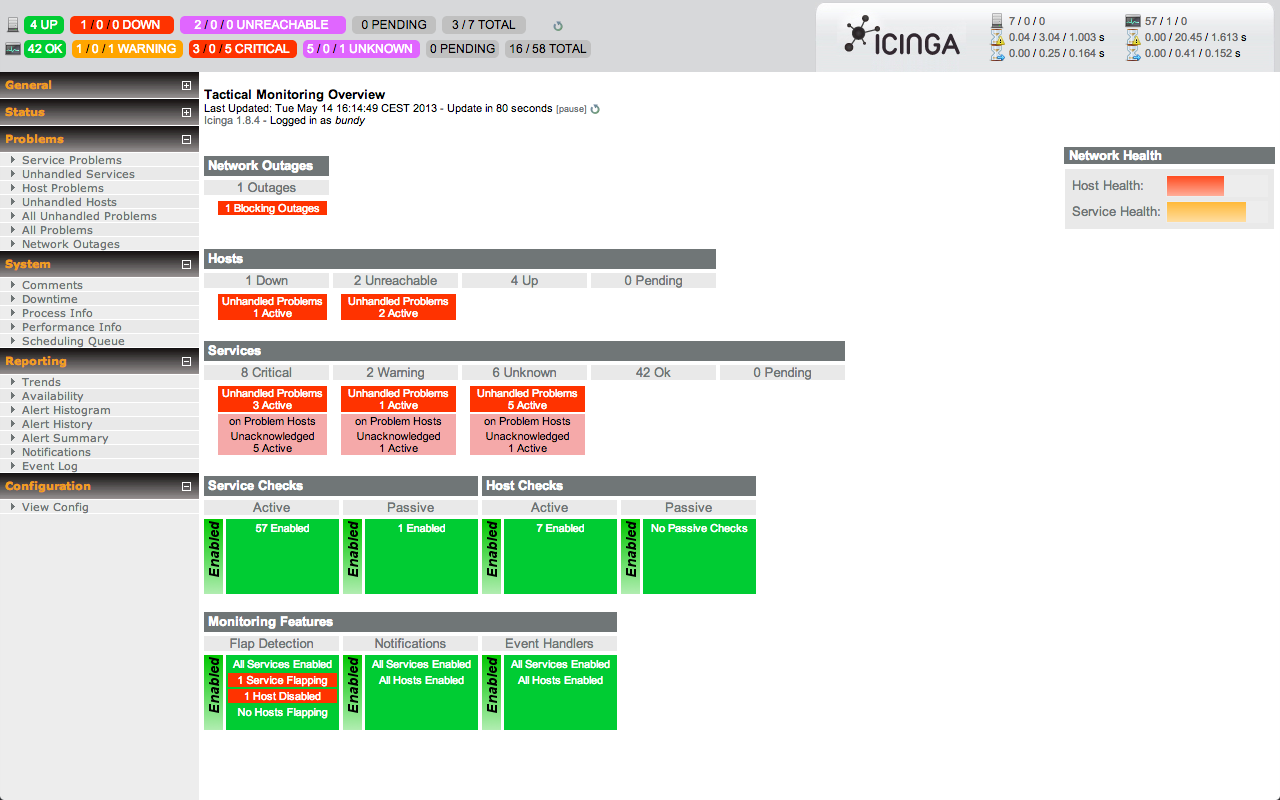
\includegraphics[scale=0.6]{img/icinga_tactical}
    \caption{En visning av "tactical overview" fra webgrensesnittet}
    \label{icingawebgui}
\end{figure}


De som sitter på servicedesk og besvarer henvendelser vil være hovedbrukerene av statusvisningen. Den skal være et hjelpemiddel for å få et overblikk over tjenester og serveres tilstand.

\subsubsection{Design}

For at statusvinduet skulle imøtekomme IKT-avdelingens ønsker, ble det besluttet å gjøre utviklingen i iterasjoner. Ofte vet ikke brukeren hva de vil ha før de ser et utkast og prosessen har begynt. For utviklingen av statusvinduet har designprosessen beskrevet i ISO 9241-210 blitt fulgt. Der er det beskrevet fire aktiviteter som går i syklus til en får et tilfredsstillende resultat:

\begin{itemize}
	\item Understand and specify the context of use
	\item Specify the user and organizational requirements
	\item Produce design solutions
	\item Evaluate designs against requirements.
\end{itemize}

Utviklingsprosessen ble startet med et møte med hele IKT-avdelingen for å presentere gruppens forslag til utkast på designet, som vist i Figur \ref{statusvindu_mockup} mockup. Her kom det frem forslag om å vise temperaturene fra serverrom-sensorene som en terning der det fysiske oppsettet kom frem.

Eksisterende programvare for denne type fremvisning ble funnet etter litt søk, og det ble besluttet å gjenbruke Nagdash cite \cite{nagdash}. Løsningen var et godt utgangspunkt for det visuelle, og er skrevet i språket PHP, noe gruppemedlemmene føler seg komfortable med og IKT-avdelingen har benyttet seg av i tidligere prosjekter. 

Nagdash baserer uthenting av informasjon om host- og serviceobjekter på nagios-api \cite{nagiosapi}, som er en tjeneste som må installeres på Icinga-serveren og setter opp et API over HTTP. Icinga har sitt eget API som det var ønskelig å benytte. Uthenting av informasjon måtte derfor endres til å bruke kall til API-et som Icinga-web tilbyr \cite{icingarestapi}.

Gjennom to iterasjoner kom det frem flere ønsker som ble lagt inn:
\begin{itemize}
	 \item Uthenting av driftsmeldinger via RSS fra portal.hedmark.org
	 \item Endre utseende for “Known Services”
	 \item Sette kolonnene med hosts og servicer ved siden av hverandre 
	 \item Hente ut og grafe antall åpne, lukkede, og mottate saker fra sakssystemet Footprints
	 \item Fjerne irrelevant informasjon som hvilket attempt en gitt service-sjekk er på
\end{itemize}

Det ble også rapportert en bug om at datoen på skjermen ikke endret seg før etter en sideoppfrisking. Koden som oppdaterer datoen var ikke lagt inn i funksjonen som sørger for automatisk oppdatering. Dette viser viktigheten av å ha brukertesting, da en slik bug kan være vanskelig å oppdage.

Etter at all funksjonalitet og design var på plass ble all kode gjennomgått av gruppen i fellesskap for å kvalitetssikre løsningen og sørge for at all ikke-triviell kode var kommentert.

I Figur \ref{statusvindu_mockup} vises en mockup av statusvisningen som vi la fram for IKT-avdelingen ved første møte.

\begin{figure}[H]
    \centering
    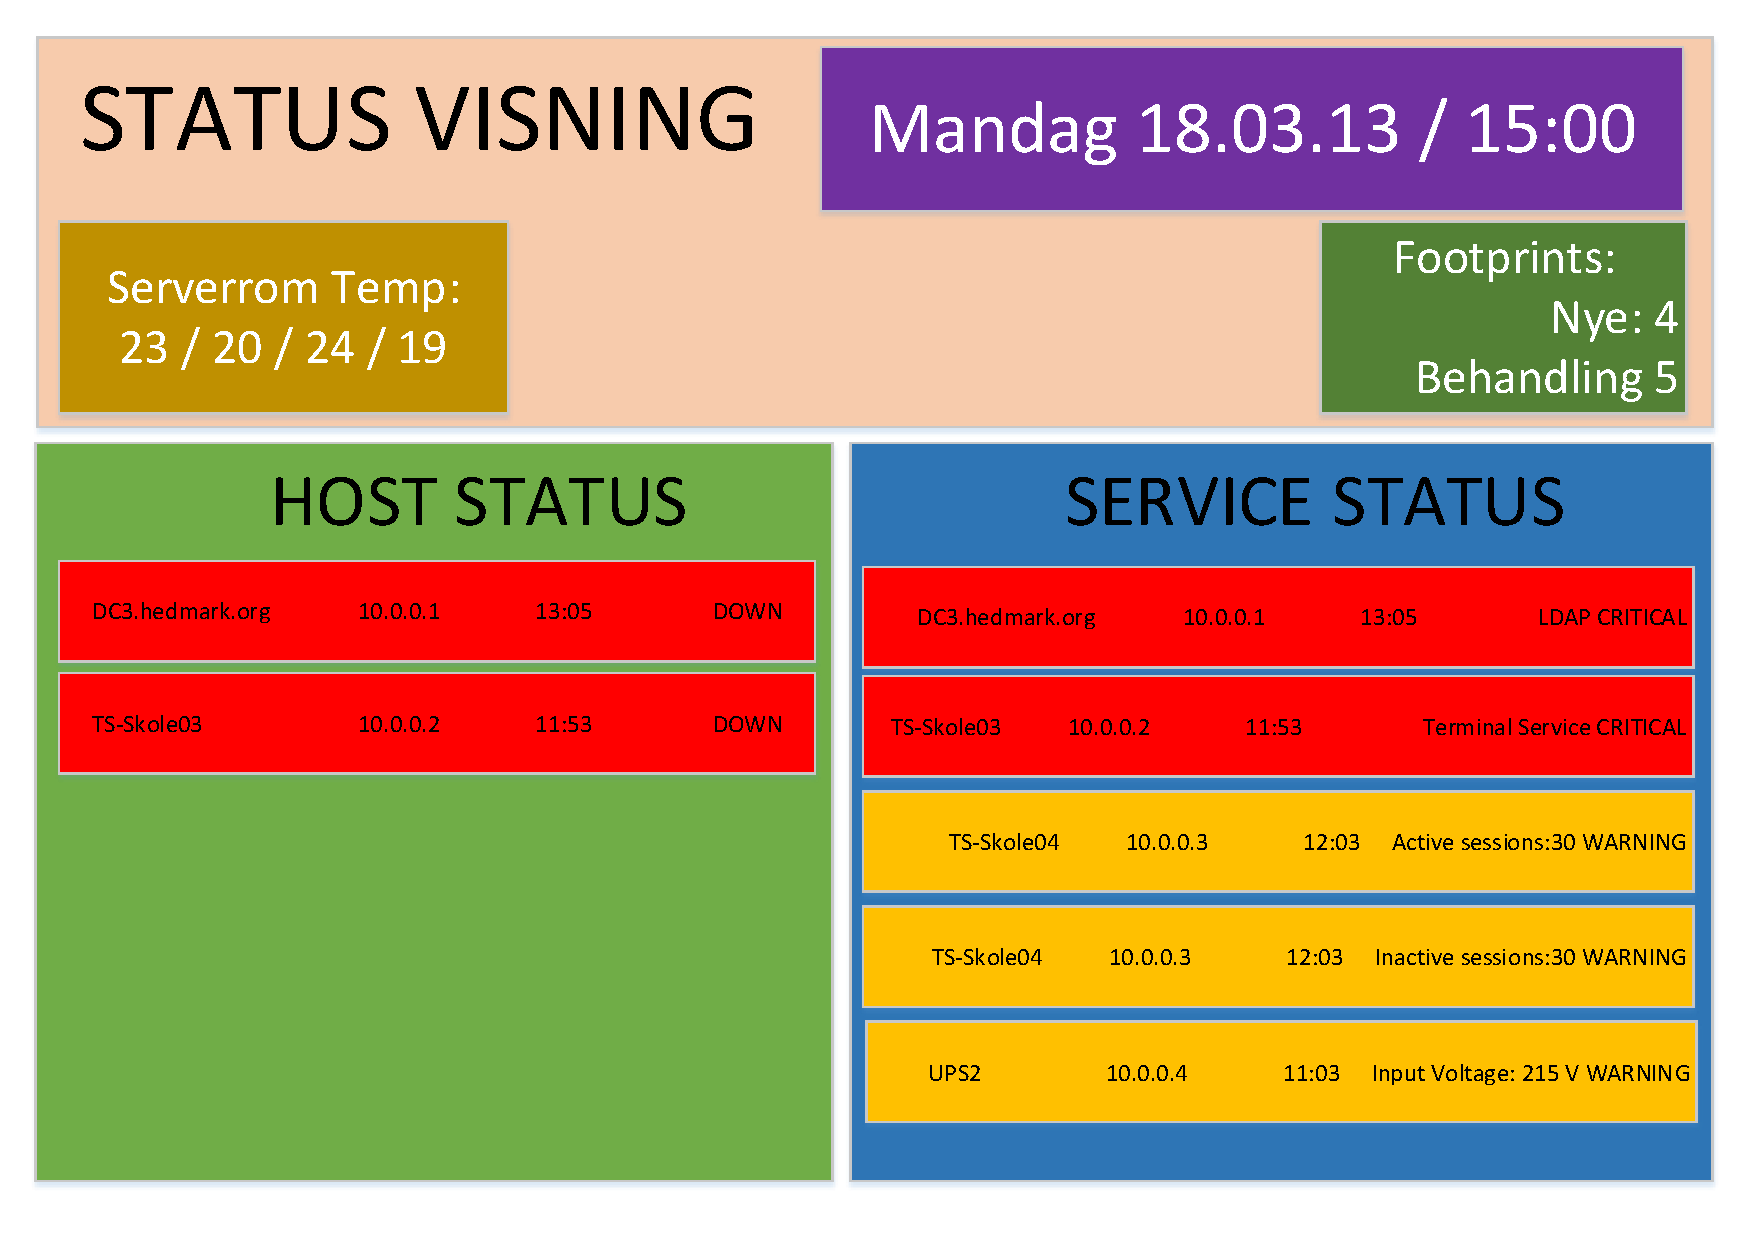
\includegraphics[scale=0.3]{img/statusvindu_mockup}
    \caption{Mockup av statusvindu}
    \label{statusvindu_mockup}
\end{figure}

Figur \ref{statusvindu_mockup} viser hvordan Nagdash ser ut med oversatte API-kall:

\begin{figure}[H]
    \centering
    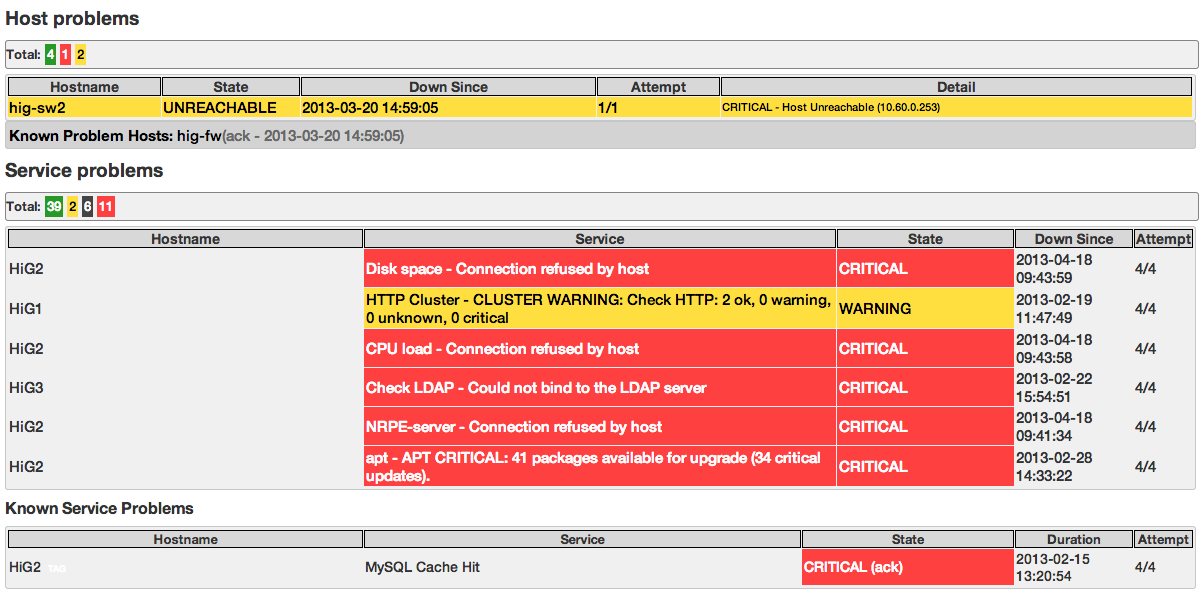
\includegraphics[scale=0.3]{img/statusvindu_oversatte_kall}
    \caption{Statusvindu med oversatte API-kall}
    \label{statusvindu_mockup}
\end{figure}


Figur \ref{statusvindu_first} viser statusvisningen etter første iterasjon, her har følgende funksjonalitet blitt lagt til:
\begin{itemize}
	\item Temperatur fra serverrommet har blitt lagt til
	\item Antall mottate og lukkede saker fra Footprints er lagt til
\end{itemize}

\begin{figure}[H]
    \centering
    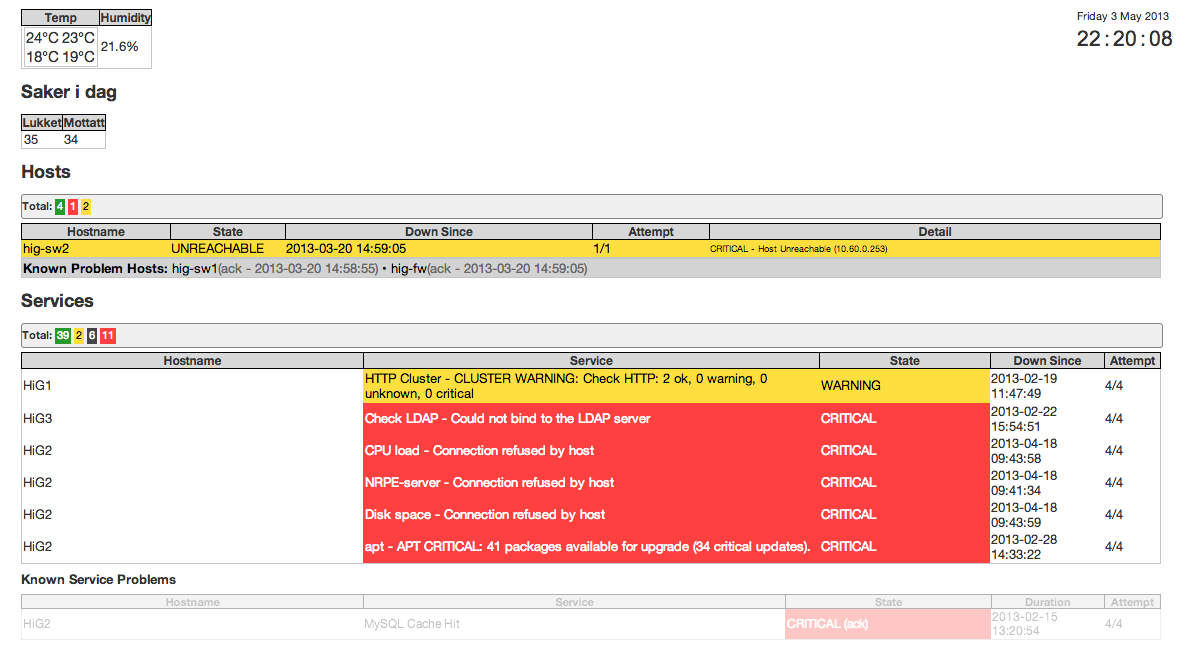
\includegraphics[scale=0.3]{img/statusvindu_first}
    \caption{Statusvindu etter første iterasjon}
    \label{statusvindu_first}
\end{figure}

Figur \ref{statusvindu_final} viser endelig statusvisningen, og her ble følgende funksjonalitet til fra første iterasjon:

\begin{itemize}
	\item Visualisering av retning på luftstrøm
	\item Temperatur fra de sensorene som er konfigurert
	\item Luftfuktighet
	\item Kolonnene for host og services er satt ved siden av hverandre
	\item Driftsmeldinger fra portal.hedmark.org
	\item Grafing av lukkede saker som er mottat i dag, lukkede saker fra alle mottate saker,
	mottate saker i dag og totalt antall åpne saker.
\end{itemize}

\begin{figure}[H]
    \centering
    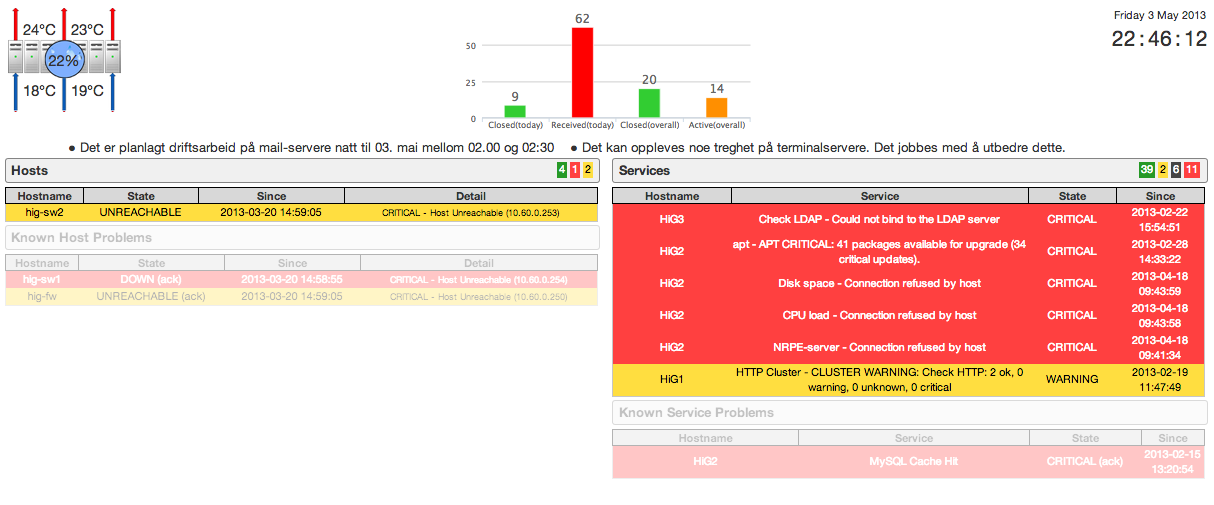
\includegraphics[scale=0.3]{img/statusvindu_final}
    \caption{Sluttresultatet av statusvinduet}
    \label{statusvindu_final}
\end{figure}


\subsubsection{Arkitektur}

Statusvindu definerer strukturen for HTML og inkluderer CSS- og Javascript.

Hver av modulene “footprints.php, netbotz.php og rss.php” retunerer et javascript-objekt med data ut fra ajax-kall fra external.js. Dataene bearbeides og settes inn i riktig “div” i html-en med javascript. Nagdash returnerer rå HTML, da denne inneholder tabeller og annen markup i tillegg til dataene.

I filen external.js hentes data fra de ulike modulene og settes inn i statusvindu dynamisk gjennom Ajax i et bestemt intervall \ref{statusvindu_arkitektur}.

\begin{figure}[H]
    \centering
    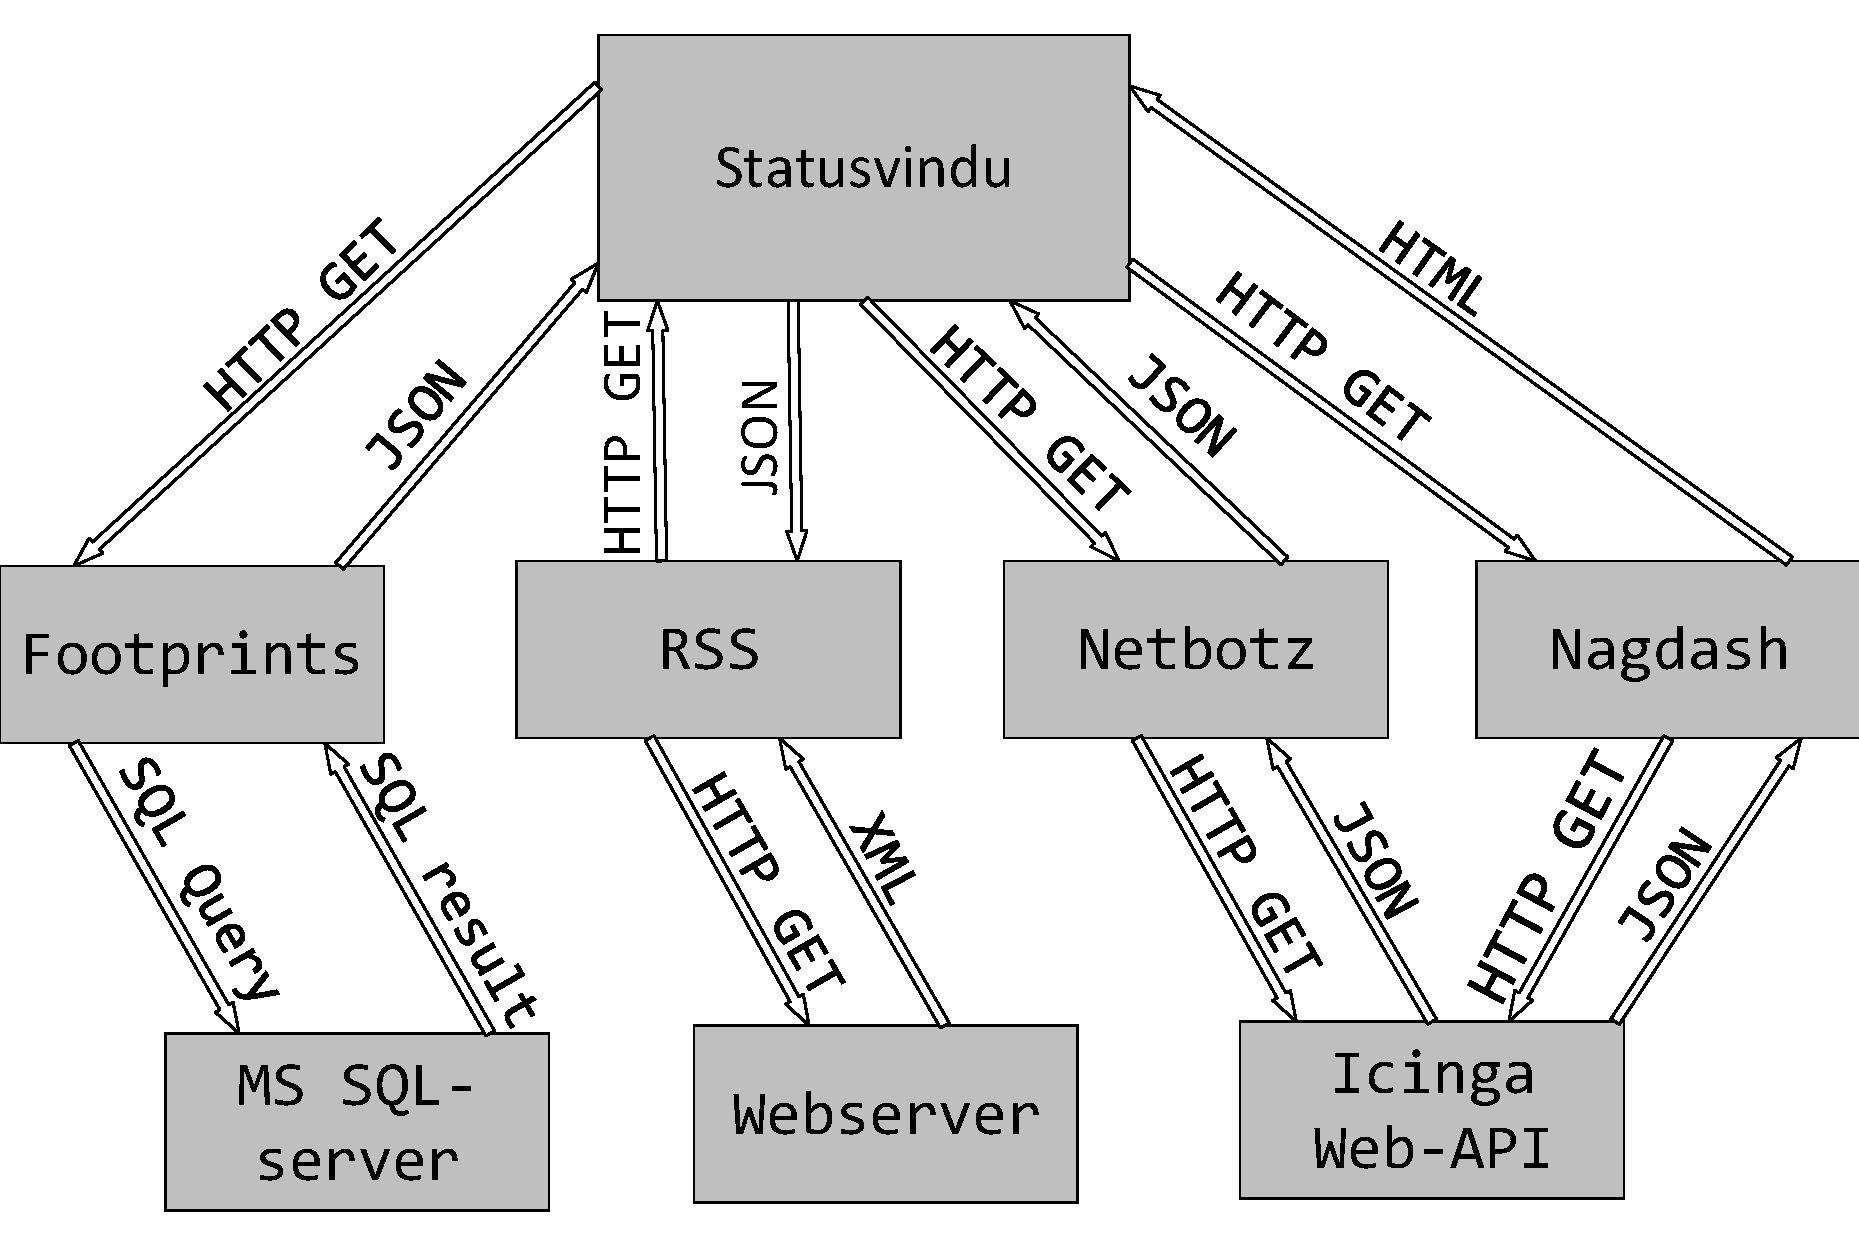
\includegraphics[scale=0.6]{img/statusvindu_arkitektur}
    \caption{Informasjonsflyt mellom modulene involvert i statusvinduet}
    \label{statusvindu_arkitektur}
\end{figure}


\subsubsection{Nagdash}

For å hente ut data fra Icinga benyttes REST-api-et til Icinga-web. I eksempelet under vises en spørring som henter alle host-objekter som har state-en DOWN (HOST\_CURRENT\_STATE|=|1) eller UNREACHABLE (HOST\_CURRENT\_STATE|=|2). Viktige parametere:
\begin{itemize}
	\item <host>: hostnavn eller IP til hosten som kjører Icinga-web
	\item <objekt>: Objekttypen spørringen skal kjøres mot (f.eks host eller service)
	\item filter: Kolonner som skal brukes i sammen med de logiske operatorene AND og/eller OR
	\item columns: kolonner som skal returneres i resultatet
	\item authkey: Nøkkelen brukt for å autentisere til API-et
\end{itemize}

\begin{lstlisting}
http://<host>/icinga-web/web/api/<objekt>/filter[OR(HOST_CURRENT_STATE|=|1;HOST_CURRENT_STATE|=|2)]/columns[HOST_ID|HOST_CURRENT_CHECK_ATTEMPT|...]/authkey=<apikey>/json
\end{lstlisting}

Da får en et javascript objekt ut med de kolonnene en har bedt om.

Vi har totalt 6 spørringer og de ulike gjør følgende:
\begin{enumerate}
	\item  hostQuery henter ut alle hosts som har status DOWN eller UNREACHABLE
	\item  serviceQuery henter ut alle servicer som har en UP host, men en service som er enten WARNING eller CRITICAL
	\item  hostTotalQuery henter ut alle hosts, med en kolonne som forteller hvilken tilstand den er i. Dette blir brukt for å regne ut et antall innen for hver tilstand.
	\item  serviceTotalQuery samme som 3., men henter alle servicer.
	\item  hostPriorityQuery henter ut en og en host basert på objekt id. Informasjonen brukes videre for å sjekke om den har en prioritets variabel satt, som vil føre til at den blir prioritert ved fremvisning.
	\item  servicePriorityQuery samme som 4., men henter her ut for en service
\end{enumerate}

\subsubsection{Footprints}

For uthenting av antallet saker innenfor ulike kategorier i Footprints ble det benyttet SQL-spørringer direkte mot databasen. IKT-avdelingen ønsket å få en graf om følgende antall om saker:
\begin{itemize}
	\item Mottat i dag
	\item Både lukket og mottat i dag
	\item Lukket av alle mottate saker
	\item Antall aktive saker
\end{itemize}

I footprints.php vil returnert data fra alle de 4 spørringene bli slått sammen til et array som videre returneres som et JSON-objekt til external.js via AJAX. 

For å grafe returnert resultat i external.js ble jQuery biblioteket Highcarts benyttet. Det ble først testet et annet bibliotek for grafing: jqBarGraph, men dette hadde manglende konfigurasjonsmuligheter.  

I utdraget nedenfor vises koden for å definere hver søyle i diagrammet (“categories”), og sette de ulike dataverdiene med stats.<variabel>:
\begin{lstlisting}
xAxis: {
   categories: ['Closed(today)', 'Received(today)', 'Closed(overall)', 'Active(overall)']

series: [{
         name: 'Amount',
         data: [{ y: stats.Closed,
                  color: '#32CD32'},
                { y: stats.Received,
             color: '#FF0000'},
                { y: stats.ClosedAll,
             color: '#32CD32'},
                { y: stats.Open,
             color: '#FF8F00'}
               ]
         }]
\end{lstlisting}

Visning søylene uten tall ga bare visualisering av forholdet mellom de ulike kategoriene, så det ble lag til konfigurasjon for å vise selve antallet over hver søyle, slik: 

\begin{lstlisting}
dataLabels: {
               enabled: true,
               style: {
                  fontSize: "16px",
                  lineHeight: "auto"
               }
\end{lstlisting}

Standard font-størrelse var for liten, så denne ble justert opp. I Internet Explorer 9.0 ble da tallet flyttet for høyt over søylen i forhold til standard høyde. En løsning på dette ble funnet via siden for rapportering av feil til Highcharts \cite{iebug} 

Endring:

\begin{lstlisting}
lineHeight: "auto"
\end{lstlisting}

Figur \ref{IE_bug} viser høydeforskjellen, høyre er før endring og venstre etter:

\begin{figure}[H]
\centering
\begin{subfigure}
  \centering
  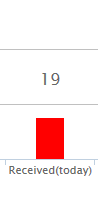
\includegraphics[scale=0.7]{img/IE_footprints_bug}
\end{subfigure}
\begin{subfigure}
  \centering
  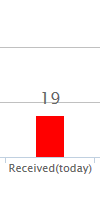
\includegraphics[scale=0.7]{img/IE_footprints_fix}
\end{subfigure}
\caption{Høydeforskjell for antall over hvert søylediagram i Internet Explorer 9.0}
\label{IE_bug}
\end{figure}



\subsubsection{Netbotz}

Det var ønskelig at det skulle være enkelt å legge til nye sensorer for temperatur og luftfuktighet. Alle sensorene oppdages automatisk av pluginen som utførerer sjekkene for Icinga. Via API-et til Icinga-web hentes siste verdi for denne sjekken ut. Samtidig får en ut hvilken ID hver av sensorene har fått. I Javascript mappes hver sensor til riktig rad.

Utdrag fra external.js
\begin{lstlisting}
 var front_layout = [2, 1]; // The netbotz sensor IDs for the front row
  var back_layout = [5, 4];  // and the back
  var columns = Math.max(front_layout.length, back_layout.length); // Largest row is used 
...
  var room = new Image(); // Set up background image for the div
  room.onload = function() {
      $('#serverroom_climate').css('width', this.width);
      $('#serverroom_climate').css('height', this.height);
      $('#serverroom_climate').css('background-image', 'url(' + this.src + ')');
   };

   // Set the background image to be one with the right number of columns
   room.src = "image.php?sensor_cols=" + columns;
\end{lstlisting}

Grafikken for servermiljø tilpasses automatisk etter den raden med flest antall sensorer, ved å lime sammen riktig antall bilder dynamisk gjennom GD i PHP. (se image.php i vedlegg x.x).

\subsubsection{RSS}

RSS-feeden hentes inn fra IKT-avdelingens egen driftsfeed, der meldinger til alle brukere legges ut. Dersom det ikke er noen meldinger vil det ikke vises noe. Hvis lengden på feeden overstiger det som får plass på én linje vil den begynne å scrolle bortover. Dette gjøres med jQuery-pluginen \cite{jqmarquee}.

\subsubsection{Prioritering}

Standard visning av et varsel er å vise den som kom inn sist øverst. Ved tilfeller der det er flere varsler, var det ønskelig å kunne gi en prioritering for å få de viktigste varslene til å komme øverst i listen. For å prioritere host-objekter som er DOWN eller UNREACHABLE og service-objekter som har WARNING eller CRITICAL i statusvisningen, ble to løsninger vurdert. 

Den ene metoden var å bruke et severity-tall som Icinga kalkulerer basert på hvor mange child-hosts og child-servicer som hører til et gitt host-objekt som er nede. Dette vises som “network outages” i Icinga Classic Web der hver host får et “severity”-tall. Det eksisterte ikke noen dokumentasjon om dette kunne hentes ut via API-et eller hvordan “severity” kalkuleres. 

Utrekningen skjer i outages.cgi, som ble funnet etter å lese gjennom HTML-koden og lese kildekoden for outages.c \cite{dnsmichi} : 
Child-servicer blir delt på et forhåndsdefinert tall (service\_severity\_divisor) som brukes for å angi hvor kritisk det er i forhold til child-hosts.

\begin{lstlisting}
temp_hostoutage->severity = (temp_hostoutage->affected_child_hosts + (temp_hostoutage->affected_child_services / service_severity_divisor));
\end{lstlisting}

Det kalkulerte tallet baseres på at hosten som er nede er parent til en eller flere andre hosts. Dette er ikke alltid tilfellet, og metoden vil da ignorere alle host-objekter som ikke er en parent. En annen svakhet er at antall services vil bli kalkulert mot en statisk variabel, som ikke nødvendigvis gjengir viktigheten.

Eksempel:
\begin{equation}
service\_severity\_divisor = 4 
\end{equation}
En host med en child-host som kjører to servicer som er viktige
\begin{equation}
Severity = 1 + (2/4) = 1.5
\end{equation}

En host med to child-hosts som kjører to servicer hver, men er ikke like viktige som nr. 1
\begin{equation}
Severity = 1 + (4/4) = 2
\end{equation}

Metoden er ikke anvendelig for prioriteringen, da det skal kunne settes på hvilken som helst service eller host, og den gjengir ikke viktigheten godt nok.     

Den andre metoden gruppen kom frem til var å sette en egendefinert variabel “\_PRIORITY” på host- og service-objekter, og å hente ut variabelen via API-et til Icinga-web.

Metoden med egendefinert variabel ble valgt, fordi denne kan anvendes på alle servicer og hosts, og gir et bedre prioriteringsgrunnlag enn severity som vurderer antall childs, noe ikke alle hosts nødvendigvis har. En kan heller ikke prioritere en service med metode 1.

Implementasjonen av metode to blir gjort ved å spørre API-et for hver host eller service som er hentet ut fra det første kallet (ref x.x). Har hosten eller servicen variabelen \_PRIORITY definert, vil denne lagres, ellers blir det satt 0 som prioritetstall.

Selve sorteringen av hosts og servicer blir gjort av PHP-funksjonen usort() med to egenskrevne sammenligningsfunksjoner. \cite{usort}. Grunnen til dette er at arrayet er flerdimensjonalt, så det må sorteres på verdien til en spesifikk nøkkel. Det skal også sorteres innenfor tilstandene DOWN og UNREACHABLE, og CRITICAL og WARNING. DOWN skal gå foran UNREACHABLE for host-objekter, og CRITICAL foran WARNING for service-objekter, deretter sorteres det etter prioriteringsvariabelen.
